\section{Methodology}
\label{sec:method}

\method{} treats reward design as a bounded interaction with tools: an agent constructs an executable reward program, tests its behavior against task-provided evidence, and revises it before reuse. The output is a program and its validation record, rather than a score for one response. We distinguish \emph{construction tools}, which help the agent design and test a program, from \emph{scoring components}, which the resulting program invokes. A single controller coordinates construction; additional specialized agents are not required.

\noindent\textbf{Scope of this revision.} We specify a revised protocol for objectively verifiable tasks, initially mathematics and code. The construction-loop comparisons and Qwen3-8B distillation below are proposed evaluations, not completed experiments. Earlier selection and RL results do not establish their effectiveness; the selection-only study is retained in Appendix~\ref{apd:legacy_routing}. Extending validation to open-ended translation and dialogue requires independent quality labels and is outside this revision's primary scope.

\subsection{Reward Construction as a Task}
\label{sec:formulation}

A construction task $\tau$ provides a specification $d_\tau$, permitted scoring resources $\mathcal{A}_\tau$, and two disjoint test suites $V_\tau^{\mathrm{dev}}$ and $V_\tau^{\mathrm{audit}}$. The specification defines the objective, input schema, available references or execution tests, and any explicit output constraints, including their priority relative to content correctness. Each suite contains response examples, oracle-derived quality labels or comparisons, and valid transformations for checking reward behavior. These labels come from task verifiers fixed before construction, not from the reward designer's own judgments. Development tests provide feedback; the audit suite remains inaccessible until the submitted program is frozen.

The agent produces a reward artifact $g_\tau$ with interface
\begin{equation}
    g_\tau(q,r,\hat r,z) \longrightarrow (s,e),
    \qquad s\in[0,1],
\end{equation}
where $q$ is a query, $r$ a response, $\hat r$ an optional training reference, and $z$ the permitted task metadata or execution tests. The structured record $e$ contains component scores and execution status. Infrastructure failures return a distinct error status rather than a valid low score. An artifact comprises source code, an applicability description, pinned dependencies, and fixed score transformations and composition parameters. References and tests are function inputs; programs may not embed development-example identifiers or answer lookup tables.

The harness consumes a stream of query records and emits one construction result per processed record. Each result stores a serialized reward definition with function-source strings, or a key into an optional content-addressed library. A key hashes the complete definition, including composition and runtime dependencies; query inputs and validation evidence are stored separately. A query without an adequate test pack can yield an unvalidated definition, but not a claim of validated reward quality.

Construction occurs at the level of a task specification or reusable task subtype. At scoring time, a router selects an applicable artifact from the library using the query and permitted metadata. It does not inspect the current candidate responses to choose their reward function. When no artifact covers the required contract, a bounded construction episode is triggered using the task's development pack.

\subsection{Modular Tools and a Fixed Reward-Model Catalogue}
\label{sec:synthesis}

The stream interface requires only structured reward definitions, task-aware validation, and submission (Table~\ref{tab:construction_tools}). General file and shell operations are optional adapters for agents that benefit from a coding workspace. Task analysis is performed by the controller from the supplied task pack; model cards are ordinary read-only resources. Neither requires a separate LLM-backed tool. Existing coding-agent file and shell interfaces can be adapted to this schema. A dedicated registry search is optional for larger libraries; small catalogues can be read directly.

\begin{table}[t]
\centering
\caption{Minimal construction interface. File and shell tools are optional and scoped to permitted resources. Versioning, validation, and registration remain harness responsibilities.}
\label{tab:construction_tools}
\small
\begin{tabularx}{\linewidth}{@{}lXX@{}}
\toprule
\textbf{Tool} & \textbf{Input} & \textbf{Observation / effect} \\
\midrule
\texttt{read\_file} & Path and bounded line range. & Content, file hash, and truncation status. \\
\texttt{write\_file} & Path, content, expected prior hash. & Updated path and content hash. \\
\texttt{edit\_file} & Path, prior hash, exact replacement. & Change record and updated hash; conflicts are explicit. \\
\texttt{run\_command} & Command, working directory, timeout. & Exit code, bounded stdout/stderr, and termination reason. \\
\texttt{test\_reward} & Serialized definition, development profile, on-pass policy. & Version-bound report; optional finalization after full admission checks. \\
\texttt{submit\_reward} & Artifact ID and validation run ID. & Acceptance or rejection and selected artifact; the driver persists the result. \\
\bottomrule
\end{tabularx}
\end{table}

\noindent\textbf{Fixed neural scoring resources.} We replace online model search, checkpoint downloading, and automatic deployment with a small, preselected catalogue $\mathcal M_0$ of representative open-source reward models, exposed through a uniform \texttt{score\_model} API. Each entry includes its model card and a versioned inference contract. The catalogue is selected before evaluation, without using target audit results, and shared by all construction baselines. Exact checkpoints and revisions belong in the experiment manifest. Inspecting a card suggests applicability; it does not certify reward quality. The agent can use these models as components, combine them with rules, or omit them. Catalogue membership stays fixed even as the library of constructed programs grows.

\noindent\textbf{Single reward and checklist modes.} The run configuration selects a single function or a checklist. In checklist mode, the agent specifies a bounded list of criteria and a source-code string for each component; the plan and all implementations can share one completion. The entire list and its aggregation form one artifact. Functions may implement answer checks, code execution against permitted tests, or calls to model APIs. A fixed runtime aggregates their normalized scores:
\begin{equation}
    s = h_\tau(q,r,z)\frac{1}{|\mathcal V|}\sum_{j\in\mathcal V} c_j\!\left(f_j(q,r,\hat r,z)\right),
    \quad \mathcal V\neq\emptyset,
\end{equation}
Here $\mathcal V$ is the set of successfully executed components. Single mode uses one function; checklist mode uses the arithmetic mean over successful components, with a bounded planned count $m$. All-component execution failure returns no score and a failed status. Coverage $|\mathcal V|/m$ and each component's status accompany partial scores. This revision does not expose trainable or agent-selected weights. Each $c_j$ maps its component to $[0,1]$ with larger values indicating better quality. Component count is bounded, and normalization, criteria, and the component list are fixed before scoring a query's candidates. The planned list is fixed, and membership in $\mathcal V$ is determined only by the declared execution-status rule, never by dropping low scores. Valid zero scores remain in the mean. Partial execution does not itself establish reward quality. The optional gate $h_\tau\in\{0,1\}$ enforces requirements explicitly present in the task; it is $1$ when no hard gate is required. Duplicate or overlapping criteria are diagnosed because repeated checks can implicitly alter emphasis even under equal averaging. Both component behavior and the final aggregate require validation; a list of executable checks alone does not establish reward quality.

\subsection{A Bounded Construction and Repair Loop}
\label{sec:routing}

An episode starts from the current query/task pack, a library snapshot, and an explicit resource budget $B$; a writable workspace is optional. The controller inspects relevant contracts, retrieves reusable artifacts, writes or adapts a candidate, and calls \texttt{test\_reward}. The harness snapshots the entire artifact before testing and binds its report to that immutable version. A failed comparison or execution error can lead to a targeted source revision and another test. Submission checks the matching full-development report; agent-written logs cannot certify acceptance. The interaction is
\begin{equation}
    a_t\sim\pi_{\mathrm{design}}(\cdot\mid C_t),
    \qquad o_t=\operatorname{Tool}(a_t),
\end{equation}
where $C_t=P_{\mathrm{run}}\Vert P_\tau\Vert h_t$ is the logical message sequence and $\Vert$ denotes concatenation. The run prefix fixes instructions and tool schemas; the episode prefix fixes the task pack, initial library snapshot, mode, and initial budget. History appends complete assistant actions, their tool observations, and updated state, including remaining budget $B_t$. Earlier messages are never rewritten. Each episode has at most one controller request in flight; independent tools may run as a batch, with results appended in call order before the next decision. Different queries have separate histories. This preserves a common prefix and permits provider-supported prefix caching without assuming a cache hit.

\noindent\textbf{Reducing model requests.} The controller can emit a plan and complete definition in one call. Tools perform lookup, hashing, batched testing, and persistence without auxiliary LLM planners or judges. Under the predeclared on-pass submission policy, \texttt{test\_reward} invokes the same trusted finalizer as explicit submission after full admission checks, eliminating a confirmation-only model turn. Repairable failures trigger further decisions. Compatible validated reuse can require zero controller calls, and a new artifact that passes immediately can require one. These are execution paths, not measured speedups; retries and neural scoring requests are counted separately (Appendix~\ref{apd:llm_protocol}).

The budget limits controller tokens, candidate submissions, and test executions; their realized costs are reported separately. Finalization selects an eligible candidate or records failure when the budget is exhausted. A retained earlier candidate must pass the same development criteria. Failed episodes remain part of the evaluation denominator. Budgets cover all checklist items and retries jointly. A supervisor enforces call and episode deadlines, limits repeated invalid/no-progress actions, and never resets the full budget for each component. Context capacity is checked before requests; exhaustion follows the same termination rule rather than silently removing history or invoking an LLM summarizer.

The outer driver owns stream iteration and durable output. Record-specific failures produce explicit results and allow subsequent queries to proceed; authentication, output-storage, or persistent infrastructure failures stop the run. EOF, cancellation, and the global budget bound the outer loop. Committed results are resumed idempotently from input/configuration digests and the recorded library state. Source persistence, execution, and isolation are separate interfaces; Docker is not required (Appendix~\ref{apd:harness_isolation}).

\begin{figure}[t]
\centering
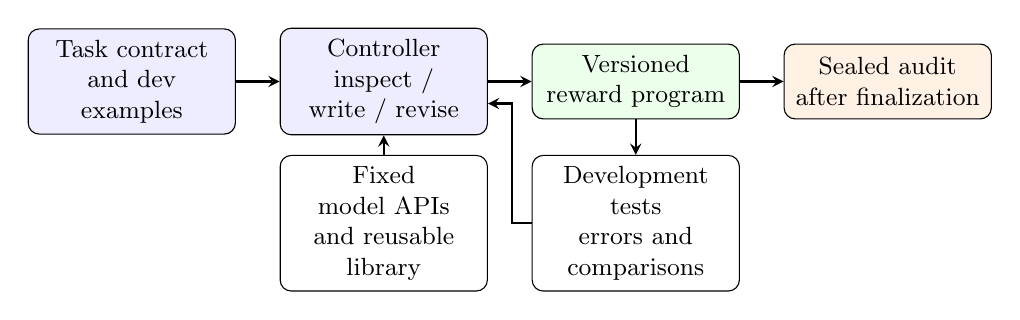
\begin{tikzpicture}[>=stealth, font=\small,
 box/.style={draw,rounded corners,align=center,text width=2.35cm,minimum height=0.95cm,inner sep=4pt},
 flow/.style={->,thick}]
\node[box,fill=blue!7] (task) at (0,0) {Task contract\\and dev examples};
\node[box,fill=blue!7] (agent) at (3.2,0) {Controller\\inspect / write / revise};
\node[box,fill=green!8] (program) at (6.4,0) {Versioned\\reward program};
\node[box,fill=orange!10] (audit) at (9.6,0) {Sealed audit\\after finalization};
\node[box] (library) at (3.2,-1.8) {Fixed model APIs\\and reusable library};
\node[box] (tests) at (6.4,-1.8) {Development tests\\errors and comparisons};
\draw[flow] (task) -- (agent);
\draw[flow] (agent) -- (program);
\draw[flow] (program) -- (audit);
\draw[flow] (library) -- (agent);
\draw[flow] (program) -- (tests);
\draw[flow] (tests.west) -- ++(-0.25,0) |- ([yshift=-0.28cm]agent.east);
\end{tikzpicture}
\caption{Revised construction loop. Development feedback supports repair; audit outcomes never return to the controller. Accepted artifacts accumulate in the library, while all interaction events are stored separately as traces.}
\label{fig:main_fig}
\end{figure}

This loop provides a testable hypothesis for agentic design: observed failures enable revisions that a single completion cannot condition on. Extra calls alone do not establish an advantage. We therefore compare against both a single completion and independent sampling under matched budgets (Section~\ref{sec:design_controls}).

\subsection{Testing the Reward Function Itself}
\label{sec:verification}

\noindent\textbf{Independent task evidence.} For mathematics, suite labels are derived from trusted answers and an independently implemented equivalence checker; for code, from trusted execution tests. The suites include correct and incorrect responses, parser edge cases, and oracle-validated perturbations. Content correctness and instruction compliance are evaluated separately. A proposed perturbation is admitted only if the task oracle confirms the intended relation; agent-generated tests are supplemental diagnostics, not a source of ground truth.

Let $P_\tau^v$ contain strictly ordered response pairs $(x^+,x^-)$ from suite $v$, where $x=(q,r,\hat r,z)$ and the task oracle prefers $x^+$ to $x^-$. Reward discrimination is
\begin{equation}
    Q_{\mathrm{rank}}^v(g)=\frac{1}{|P_\tau^v|}
       \sum_{(x^+,x^-)\in P_\tau^v}
       \mathbf{1}\{g_s(x^+)>g_s(x^-)\},
\end{equation}
where $g_s$ denotes the scalar output. Ties and execution failures do not pass a strict comparison. For pairs $E_\tau^v$ whose quality should be unchanged under the task contract, we also measure
\begin{equation}
    Q_{\mathrm{inv}}^v(g)=\frac{1}{|E_\tau^v|}
       \sum_{(x,x')\in E_\tau^v}
       \mathbf{1}\{|g_s(x)-g_s(x')|\leq\epsilon_\tau\}.
\end{equation}
The tolerance is fixed before comparison, and errors count as failures. Unchanged-quality examples may include equivalent numeric representations or permitted whitespace changes; strict comparisons include wrong-answer substitutions and confirmed code mutations. Constant rewards can pass invariance tests but fail discrimination, so neither metric is sufficient alone.

\noindent\textbf{Acceptance and audit.} We report a vector of execution success, ranking accuracy, invariance, constraint violations, and false acceptance/rejection rates at a development-fixed score threshold. Task-specific minimum coverage and acceptance thresholds are predefined on training/development tasks and shared by all methods. An artifact is registered only if its interface and required development criteria pass; this constitutes development validation, not proof of general correctness. The frozen final artifact is evaluated once on the sealed audit suite. Audit outcomes cannot guide repair, registration, or candidate selection. Split provenance, mutation families, and thresholds are detailed in Appendix~\ref{apd:construction_protocol}.

A strong objective verifier may already be an effective reward. Whenever it is available under the scoring contract, \emph{direct oracle reward} is a required baseline. We do not create an advantage by withholding an otherwise available checker from competing methods. Construction is useful only if it improves measurable quality, coverage, or cost over such direct use; downstream RL is needed to determine whether better offline diagnostics improve policy learning.

\subsection{Minimal Memory and Consistent RL Scoring}
\label{sec:library_memory}

The runtime retains only an episode workspace and a persistent artifact library $\mathcal F$. Each library entry stores code and version, applicability, dependencies, calibration, development-test provenance, and a short validation report. Tags and text matching suffice for retrieval. Equivalent source/configuration hashes are deduplicated, revisions receive new versions, and previously accepted artifacts are immutable. Raw transcripts remain in the trace store rather than becoming an additional long-term memory system. Evaluation splits cannot share test-derived artifacts.

For a query $q$, the router selects or constructs one artifact $g_q$ before scoring its rollout group $\{r_i\}_{i=1}^{G}$. All candidates use the same artifact version, scoring components, calibration, and equal-mean aggregation:
\begin{equation}
    s_i=g_{q,s}(q,r_i,\hat r,z),\qquad
    A_i=\frac{s_i-\bar s}{\operatorname{std}(s)+\epsilon_{\mathrm{adv}}}.
\end{equation}
Zero-variance groups receive zero advantages. Candidate-caused failures, such as invalid code or a candidate exceeding its execution limit, follow the task contract; infrastructure/API failures are logged separately. With partial execution, a candidate uses the mean of its successful components and records their mask. Different masks can affect group comparability; coverage and missingness patterns must therefore be evaluated separately. If all components fail for a candidate, its score is invalid and the downstream group follows a predeclared retry/fallback or omission policy, rather than treating failure as zero. Function updates take effect only for a subsequent rollout batch; rewards are not recomputed midway through optimization of an existing batch.

\subsection{Recorded Traces and Learning to Design Rewards}
\label{sec:trace_learning}

We record every observable construction event, including task and split IDs, the library snapshot, controller/model versions, tool arguments and results, source patches, test reports, finalization status, tokens, latency, and cost. Brief explicit design notes can be logged, but the trace does not depend on access to hidden model reasoning. Failures and repairs are retained, and versioned observations support replay. Audit records are stored separately and excluded from the controller history.

To test whether Qwen3-8B can learn this capability, a stronger teacher collects construction traces on training tasks. Successful development-validated traces, including their failed intermediate attempts and subsequent repairs, supply supervised targets for tool selection, arguments, code edits, and final submission. Training applies next-token loss only to assistant actions and program outputs; tool observations are conditioning context, not prediction targets. Task families/templates and their derived examples are split before trace collection and library construction. No held-out-task artifacts or audit feedback enter student training.

The student is evaluated as a reward designer with the same APIs, initial library, and budget as the teacher. It is distinct from any Qwen3-8B policy trained downstream using the resulting rewards. Comparisons include the untrained student, final-program-only SFT, full-trace SFT, and the teacher. Primary outcomes are held-out reward quality, successful construction rate, repair after observed failures, and construction cost, rather than imitation of the teacher's wording. This protocol tests learnability; no successful distillation result is assumed.

\subsection{Comparisons That Isolate Agentic Construction}
\label{sec:design_controls}

The primary baseline uses one chat completion to produce an executable reward artifact. It receives the same task pack, initial library, model cards, permitted scoring APIs, and labeled development examples as the agent; it receives no feedback from executing its own draft. Every submitted artifact is scored by the same external harness. We additionally compare budget-matched independent drafts selected by a fixed development evaluator, and multi-turn self-revision without execution observations. These separate adaptive use of feedback from increased sampling or generation budget.

Reward representation (single versus checklist) is crossed with construction strategy; checklist component evaluations count toward the same total budget. Module ablations remove execution feedback, persistent-library reuse, custom code construction, or neural scoring APIs one at a time. The no-execution-feedback condition also disables construction-time Bash and interactive scoring calls; removing only \texttt{test\_reward} measures the value of standardized validation while leaving self-written execution feedback available. Fixed versus accumulating libraries are compared on identically ordered construction streams with separate, uncontaminated audit sets. All variants use the same resource accounting, failure handling, and final evaluation. We report per-task metrics and quality--cost tradeoffs; any superiority over single-turn design is an empirical question. Appendix~\ref{apd:construction_protocol} specifies the controls and trace protocol.
